\section{Cache Mapping}

Modern systems subdivide both RAM and cache into equally sized blocks (often called \textit{lines}). For instance, a 64\,B block is commonly used: when a byte is requested, the entire 64\,B block containing that byte is fetched into the cache. This approach reduces the overhead of fetching data from memory and exploits spatial locality.

\begin{figure}[H]
    \centering
    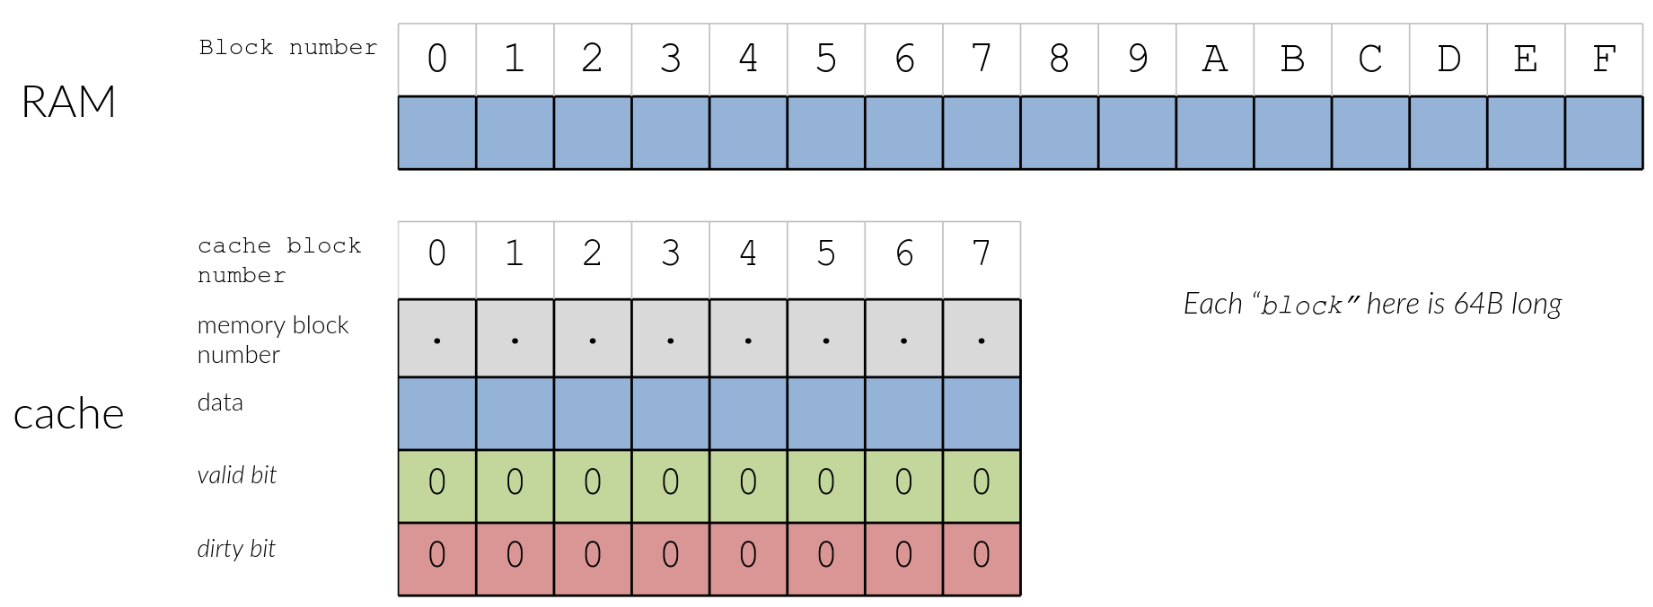
\includegraphics[width=0.8\textwidth]{assets/cache_mapping.png}
    \caption{Main memory and cache are both split into blocks (lines).}\label{fig:cache_mapping}
\end{figure}

There are three primary strategies for mapping main memory blocks into cache:

\begin{itemize}
    \item \textbf{Fully Associative Mapping}
    \item \textbf{Direct Mapping}
    \item \textbf{N-way (Set) Associative Mapping}
\end{itemize}

Each strategy differs in how flexible it is in placing a main memory block into cache and how it handles conflicts when multiple blocks compete for the same cache location. A high-level comparison is shown in \cref{fig:cache_mapping_ways}.

\begin{center}
    \begin{minipage}{0.2\textwidth}
        \centering
        \small
        \textbf{Fully Associative}
    \end{minipage}%
    \hspace{0.55em}
    \begin{minipage}{0.2\textwidth}
        \centering
        \small
        \textbf{Direct Mapping}
    \end{minipage}%
    \hspace{0.55em}
    \begin{minipage}{0.2\textwidth}
        \centering
        \small
        \textbf{N-way Associative}
    \end{minipage}
    \hspace{0.3em}
\end{center}

\vspace{-1em}

\begin{figure}[H]
    \centering
    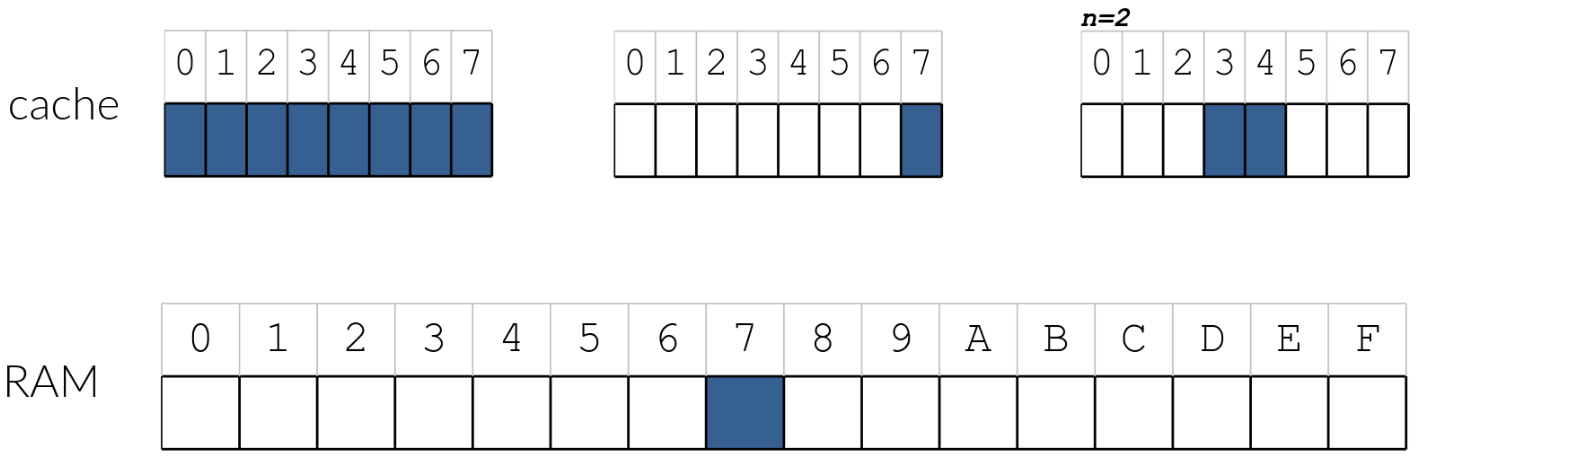
\includegraphics[width=0.77\textwidth]{assets/cache_mapping_ways.png}
    \caption{Fully Associative, Direct, and N-way Set Associative mappings.}\label{fig:cache_mapping_ways}
\end{figure}

\subsubsection{Fully Associative Mapping}
In a \textbf{fully associative} cache, each block of main memory \bfit{can be placed in any block} of the cache. This offers maximum flexibility because there is no restriction on which cache line a particular memory block can occupy. However, this scheme also requires more complex hardware for searching (to locate a given address in any cache line), making it more expensive.

\begin{minipage}[t]{0.48\textwidth}
    \textbf{Pros}
    \begin{itemize}
        \item Minimizes conflicts during \textit{writes}, as any free cache line can be used.
        \item Offers the greatest flexibility in block placement.
    \end{itemize}
\end{minipage}\hspace{1em}
\begin{minipage}[t]{0.48\textwidth}
    \textbf{Cons}
    \begin{itemize}
        \item Potentially inefficient for \textit{reads} because the requested data could be in any cache line, requiring a more expensive search mechanism (e.g., parallel or associative search).
        \item Higher hardware complexity and cost (larger tag comparators, fully associative lookups).
    \end{itemize}
\end{minipage}

\subsubsection{Direct Mapping}
In a \textbf{direct-mapped} cache, each block of main memory \bfit{can be placed in exactly one block} of the cache. This mapping is determined by some bits of the memory address (e.g., index bits), which directly select the cache line. It is the simplest scheme in terms of hardware.

\begin{minipage}[t]{0.48\textwidth}
    \textbf{Pros}
    \begin{itemize}
        \item Very efficient in locating or writing data because each memory block maps to a single known location (no associative search needed).
        \item Simpler and cheaper hardware implementation.
    \end{itemize}
\end{minipage}\hspace{1em}
\begin{minipage}[t]{0.48\textwidth}
    \textbf{Cons}
    \begin{itemize}
        \item Maximizes cache conflicts when multiple addresses map to the same cache line (known as \textit{conflict misses}).
        \item A single cache line might be heavily contended by multiple memory blocks, reducing overall hit rate.
    \end{itemize}
\end{minipage}

\subsubsection{N-way Set Associative Mapping}
In an \textbf{N-way set associative} cache, the cache is divided into sets, each containing $N$ lines. A block of main memory \bfit{can be placed in any of the $N$ lines} within the specific set dictated by the address. This approach strikes a balance between fully associative and direct-mapped schemes.


\begin{minipage}[t]{0.48\textwidth}
    \textbf{Pros}
    \begin{itemize}
        \item Reduces conflict misses compared to direct mapping by allowing multiple possible lines in each set.
        \item Lower hardware complexity than fully associative (search is limited to $N$ lines in the set, not the entire cache).
    \end{itemize}
\end{minipage}\hspace{1em}
\begin{minipage}[t]{0.48\textwidth}
    \textbf{Cons}
    \begin{itemize}
        \item More complex than direct mapping (requires searching up to $N$ lines in the set).
        \item Additional hardware and logic needed to manage the multiple lines per set.
    \end{itemize}
\end{minipage}

The choice of cache mapping strategy involves a trade-off between hardware complexity, access speed, and conflict rate.

\dots

